\chapter{Pengantar Big O dan Model Matematika}\label{ch:modul1}

\section{Pendahuluan}
Algoritma merupakan langkah-langkah yang ditempuh untuk menyelesaikan masalah. Ada sebuah, atau sekumpulan, input yang diproses sehingga menghasilkan sebuah (atau sekumpulan) output ataupun kondisi yang didefinisikan sebagai solusi untuk masalah di awal. Langkah-langkah yang ditempuh, bertujuan untuk mentransfer logika manusia dalam menyelesaikan masalah komputasi, ke dalam program komputer.

Masalah komputasi tidak hanya dapat diselesaikan dengan sebuah cara. Bisa jadi, ada banyak jenis cara atau algoritma yang dapat menyelesaikan sebuah pokok permasalahan yang sama. Sebagai contoh, masalah pengurutan dapat diselesaikan dengan algoritma Bubble Sort, Merge Sort, dan berbagai algoritma yang lain.

\section{Kompleksitas Algoritma}
Algoritma yang berbeda tentu saja memiliki langkah-langkah yang berbeda. Sehingga, ada algoritma yang lebih �cepat� dibandingkan algoritma yang lain. Dan ada pula algoritma yang lebih �hemat� dalam penggunaan memori. Algoritma yang baik adalah algoritma yang dapat menyelesaikan masalah  sekaligus efisien dalam pemakaian waktu dan ruang. Istilah yang digunakan untuk mengukur hal tersebut adalah \textbf{kompleksitas algoritma}. Maka, terdapat 2 jenis kompleksitas algoritma, yakni:

\begin{itemize}
    \item kompleksitas waktu ($T(n)$), dan
    \item kompleksitas ruang ($S(n)$).
\end{itemize}

Tentu diperlukan sebuah metode untuk mengukur seberapa �cepat�-kah sebuah algoritma atau seberapa �hemat�-kah pemakaian ruang memori algoritma tersebut. Menganalisis sebuah algoritma mencakup menganalisis kompleksitas algoritma. Meskipun terdapat 2 jenis kompleksitas, dalam analisis algoritma yang lebih difokuskan adalah analisis �kecepatan� algoritma tersebut, atau kompleksitas waktunya ($T(n)$).

�Cepat � lambat� sebuah algoritma tidak dihitung menggunakan satuan waktu yang umum digunakan dalam kehidupan, seperti detik, menit, ataupun jam. Alasannya karena kecepatan proses sebuah algoritma yang sudah diimplementasikan ke dalam program komputer bergantung pada banyak faktor, seperti processor, sistem operasi, compiler yang digunakan, dan faktor lain. Menghitung komplksitas waktu sebuah algoritma adalah \textbf{menghitung jumlah langkah yang ditempuh, serta perubahan jumlah langkah saat ukuran input berubah}. Jadi, tidak aka nada hubungannya dengan performa komputer atau kompiler yang digunakan sebagai media implementasi algoritma tersebut.

\section{Notasi Asimtotik}

Sebagaimana dijelaskan pada sub-bagian di atas, untuk mengukur kompleksitas waktu algoritma tidak digunakan satuan waktu yang umum. Maka, dibutuhkan sebuah notasi khusus. Notasi matematis yang digunakan disebut \textbf{notasi asimtotik}. Notasi asimtotik digunakan untuk melihat seberapa efisien performa sebuah algoritma bila dibandingkan dengan algoritma yang lain. 

Terdapat beberapa jenis notasi asimtotik dalam bidang ilmu matematika yang digunakan dalam pengukuran kompleksitas algoritma. 3 contoh jenis notasi asimtotik adalah:

\begin{enumerate}
    \item O (Big-O)
    \item $\Omega$ (Big-Omega)
    \item $\Theta$ (Big-Theta)
\end{enumerate}

Dalam modul ini tidak akan dijelaskan secara terperinci bagaimana menggunakan masing-masing notasi. Namun, yang akan dijelaskan adalah bagaimana kompleksitas waktu sebuah algoritma dapat ditemukan dengan menggunakan notasi tersebut.

Notasi yang paling umum digunakan adalah O (Big-O). Alasannya adalah karena notasi tersebut digunakan untuk menggambarkan batas atas (\textit{upper limit}) dari sebuah fungsi ketika masukan untuk fungsi tersebut meningkat (\textit{increase}). Alhasil, Big-O sangat cocok untuk memperlihatkan \textit{worst case} dari sebuah algoritma. Apa yang dimaksud dengan worst case akan dijelaskan pada salah satu sub-bagian dari modul ini.

Contoh penggunaan Big-O: Algoritma Bubble Sort. $T(n) = O(n^2)$. Artinya: algoritma Bubble Sort memiliki kompleksitas waktu $n^2$. 

\section{Mengukur Kompleksitas Algoritma Menggunakan Big-O}

Cara menghitung kompleksitas algoritma non rekursif tidak persis dengan algoritma rekursif. Namun yang pasti adalah, bahwa penggunaan fungsi matematis dan aturan dasar penjumlahan digunakan dalam perhitungan.

Pada setiap modul, seraya berbagai teknik desain algoritma akan dibahas, juga akan diperlihatkan bagaimana menghitung kompleksitas algoritmanya. 

Secara umum, langkah-langkah untuk mengukur kompleksitas algoritma non rekursif (umum):

\begin{enumerate}
    \item Mengidentifikasi operasi dasar
    \item Menentukan ukuran input.
    \item Memeriksa apakah pertumbuhan operasi dasar hanya bergantung pada ukuran input. Jika ya, maka tidak ada \textit{worst case} ataupun \textit{best case}. Namun jika terdapat faktor lain, maka perhitungan \textit{worst case} dibedakan dengan \textit{best case}.
    \item Menghitung derajat pertumbuhan langkah operasi dasar terhadap perubahan ukuran input dengan menggunakan fungsi matematika.
\end{enumerate}

Beberapa rumus matematika yang umum digunakan:

\begin{enumerate}
    \item $\sum\limits_{i=l}^u 1 = 1 + 1 + 1 + 1 + \ldots = u - l + 1$
    \item $\sum\limits_{i=1}^n 1 = n$
    \item $\sum\limits_{i=1}^n i = 1 + 2 + \cdots + n = \frac{n(n + 1)}{2} \approx \frac{1}{2}n^2$
    \item $\sum\limits_{i=1}^n i^2 = 1^2 + 2^2 + \cdots + n^2 = \frac{n(n + 1)(2n + 1)}{6} \approx \frac{1}{3}n^3$
    \item $\sum\limits_{i=1}^n i^k = 1^k + 2^k + \cdots + n^k \approx \frac{1}{k + 1}n^{k+1}$
    \item $\sum\limits_{i=0}^n a^i = 1 + a + \cdots + a^n = \frac{a^{n + 1} - 1}{a - 1}(a \neq 1)$
    \item $\sum\limits_{i=0}^n 2^i = 2^{n + 1} - 1$
    \item $\sum\limits_{i=1}^n i \times 2^i = 1 \times 2^1 + 2 \times 2^2 + \cdots + n \times 2^n \approx \frac{1}{3}n^3$
    \item $\sum\limits_{i=l}^u ca_i = c \sum\limits_{i=l}^u a_i$
    \item $\sum\limits_{i=l}^u (a_i \pm b_i) = \sum\limits_{i=l}{u} a_i \pm \sum\limits_{i=l}{u} b_i$
\end{enumerate}

Contoh sederhana:

\lstinputlisting[language=Python, caption=Maximum Element]{code/1-max-element.py}

\FloatBarrier

\begin{enumerate}
    \item \textbf{Mengidentifikasi operasi dasar.} Operasi dasar adalah perbandingan antara \textbf{max} dan \textbf{A[i]}, karena itulah operasi yang paling sering dilakukan yang merupakan logika dasar algoritma tersebut untuk memecahkan masalah.
    \item \textbf{Menentukan ukuran input.} Ukuran input adalah \textbf{n}, yang merupakan besar / panjang dari array atau list \textbf{A}. \textbf{n} menjadi ukuran input karena berpengaruh terhadap banyaknya operasi dasar dilakukan.
    \item \textbf{Memeriksa apakah pertumbuhan operasi dasar hanya bergantung pada ukuran input.} Untuk algoritma di atas, \textbf{n} merupakan satu-satunya penentu banyaknya operasi dasar dilakukan, sehingga dalam perhitungan kompleksitas tidak diikutsertakan analisis \textit{worst case}, \textit{best case}, maupun \textit{average case}.
    \item \textbf{Menghitung derajat pertumbuhan langkah operasi dasar terhadap perubahan ukuran input dengan menggunakan fungsi matematika.} Di bawah ini merupakan cara perhitungannya.
\end{enumerate}

\lstinputlisting[language=Python, 
                 caption=Perulangan pada Maximum Element, 
                 linebackgroundcolor={\ifnum\value{lstnumber}>5\ifnum\value{lstnumber}<11\color{codehighlight}\fi\fi}
                ]
                {code/1-max-element.py}

\FloatBarrier

$$
T(n) = \sum\limits_{i=0}^{n-1} 1
$$

Penjelasan: Perulangan merupakan deret, sehingga perulangan yang terpola dengan baik dapat digantikan ke dalam rumus matematis di atas. Isi dari sigma berisi 1 karena: \textbf{dalam setiap perulangan terdapat 1 kali operasi dasar dilakukan}.

$$
T(n) = n - 1 + 1 = n
$$

Penjelasan: Gunakan rumus pertama yang tertera sebelum contoh algoritma.

$$
T(n) = O(n)
$$

Penjelasan: Hasil akhir diubah ke dalam notasi asimtotik sesuai dengan aturan notasi.

Alhasil, algoritma di atas memiliki kompleksitas O(n), atau sering disebut dengan kompleksitas linear. Terdapat beberapa pengelompokan kompleksitas yang umum.

\section{Kriteria Efisiensi umum}

Terdapat beberapa kriteria efisiensi umum:

\begin{enumerate}
    \item \textbf{$O (1)$: Kompleksitas Konstan.} Merupakan kriteria di mana ukuran input sama sekali tidak berpengaruh pada jumlah langkah sebuah algoritma. Kompleksitas ini merupakan jenis yang paling efisien / cepat.
        
    \begin{figure}
        \centering
        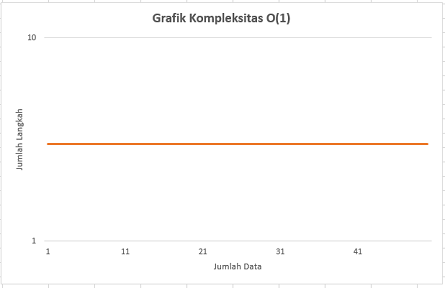
\includegraphics[width=\textwidth]{fig/ConstantGrowth}
        \caption{Testing}
    \end{figure}

    \FloatBarrier

    \item \textbf{$O (\log n)$: Kompleksitas Logaritmik.} Merupakan kompleksitas di mana perubahan / peningkatan besar dari ukuran input hanya memberikan sedikit sekali pengaruh terhadap pertumbuhan jumlah langkah. Algoritma yang memiliki kompleksitas logaritmik sering dijumpai pada algoritma yang dibuat dengan teknik divide \& conquer yang akan dibahas pada salah satu modul.

    \begin{figure}
        \centering
        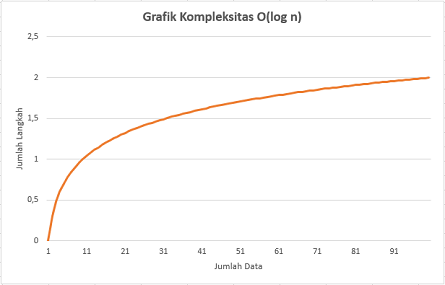
\includegraphics[width=\textwidth]{fig/LogarithmicGrowth}
        \caption{Testing}
    \end{figure}

    \FloatBarrier

    \item \textbf{$O (n)$: Linear.} Merupakan kompleksitas algoritma di mana pertumbuhan ukuran input sebanding dengan pertumbuhan jumlah langkah. Algoritma dengan kompleksitas linear dipandang sebagai algoritma yang cepat / efisien, meskipun itu juga bergantung pada permasalahan apa yang diselesaikan oleh sebuah algoritma.

    \begin{figure}
        \centering
        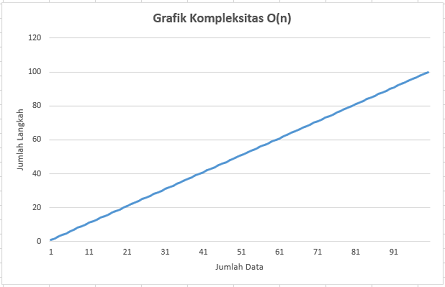
\includegraphics[width=\textwidth]{fig/LinearGrowth}
        \caption{Testing}
    \end{figure}

    \FloatBarrier

    \item \textbf{$O (n \log n)$.} Kompleksitas ini belum memiliki nama khusus. Jenis kompleksitas ini juga sering dijumpai pada algoritma yang berbasis teknik divide \& conquer. Hanya saja, pada kompleksitas jenis ini, perubahan jumlah langkah sedikit lebih besar daripada kompleksitas linear.

    \begin{figure}
        \centering
        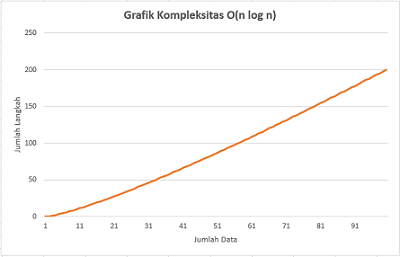
\includegraphics[width=\textwidth]{fig/NLogNGrowth}
        \caption{Testing}
    \end{figure}

    \FloatBarrier

    \item \textbf{$O (n^m)$: Kompleksitas Polinomial.} Merupakan jenis kompleksitas yang tinggi. $O (n^2)$ disebut dengan kompleksitas kuadratik. Merupakan jenis kompleksitas di mana sedikit perubahan pada ukuran input akan berpengaruh besar pada jumlah langkah.

    \begin{figure}
        \centering
        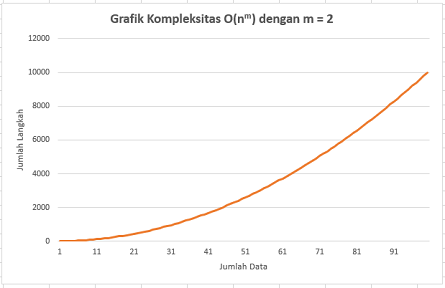
\includegraphics[width=\textwidth]{fig/ExponentialGrowth}
        \caption{Testing}
    \end{figure}

    \FloatBarrier

    \item \textbf{$O (n!)$: Kompleksitas faktorial.} Merupakan jenis kompleksitas yang sangat tinggi. Sedikit perubahan pada ukuran input akan berpengaruh sangat besar terhadap jumlah langkah. Kompleksitas ini sangat dihindari, namun untuk sebuah permasalahan komputasi yang sangat kompleks algoritma dengan kompleksitas yang tinggi juga sering digunakan.
\end{enumerate}

\begin{figure}
    \centering
    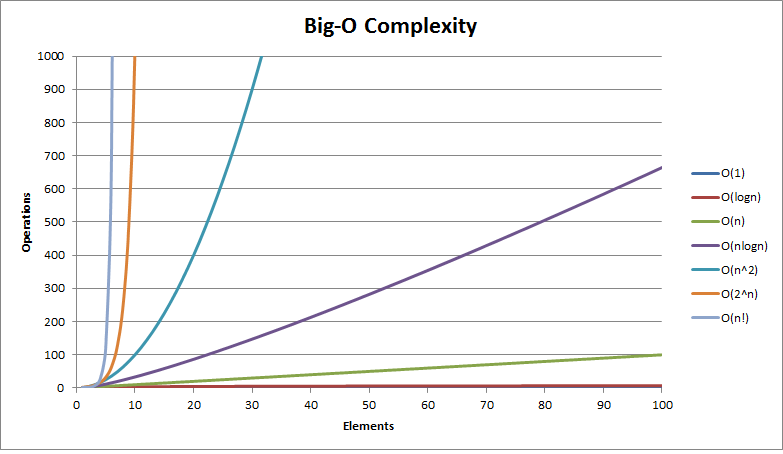
\includegraphics[width=\textwidth]{fig/AllComplexityComparison}
    \caption{Testing}
\end{figure}

    \FloatBarrier

\section{Worst Case, Average Case, dan Best Case}

Dalam pengukuran kompleksitas algoritma, terdapat \textit{worst case}, \textit{average case}, dan \textit{best case}.

\begin{enumerate}
    \item Best case / kasus terbaik: merupakan kondisi di mana algoritma akan bekerja dengan kompleksitas paling rendah untuk ukuran input yang sama. 
    \item Worst case / kasus terburuk: merupakan kebalikan dari kasus terbaik, di mana algoritma akan bekerja dengan kompleksitas tertinggi untuk ukuran input yang sama.
    \item Average case / kasus rata-rata: merupakan kondisi yang paling sering terjadi untuk sebuah permasalahan.
\end{enumerate}

% Bagian ini nanti perlu diperbaiki / disusun ulang lagi
% supaya bacanya make sense. Sementara merging punya Vincent dulu.
\section{Pengenalan Kompleksitas Algoritma}
Waktu yang diperlukan bagi \textit{Insertion Sort} untuk menyelesaikan proses pengurutannya tergantung pada jumlah masukan. Dengan kata lain, semakin besar jumlah masukan, semakin lama waktu yang diperlukan. Untuk dua masukan dengan jumlah yang sama, \textit{Insertion Sort} bisa memakan waktu yang berbeda tergantung dari seberapa terurutnya mereka. Dari sini, kita bisa mengambil kesimpulan bahwa, waktu yang diperlukan berkembang sesuai dengan ukuran dari masukan.

Besar masukan sebuah algoritma sangat tergantung terhadap permasalahan yang sedang dihadapi. Sebagai contohnya, jika berbicara mengenai permasalahan pengurutan maka besar masukan berupa berapa banyak bilangan dalam sebuah \textit{array} (\textit{array size}). Untuk permasalahan lain seperti misalnya permasalahan pencarian rute terpendek dimana masukannya adalah berupa \textit{graph} (akan dijelaskan di mata kuliah struktur data), maka yang menjadi besar masukannya adalah jumlah \textit{vertice} dan \textit{edge} dari \textit{graph} tersebut. 

\section{Analisis algoritma}
Untuk mengetahui seberapa effisien sebuah algoritma bisa dilakukan setelah menganalisis kompleksitas dari algoritma tersebut. Melakukan analisis algoritma berarti memprediksi berapa sumber daya (misalnya berapa lama waktu eksekusi atau berapa besar memori yang dibutuhkan) yang dibutuhkan oleh sebuah program ketika mengeksekusi algoritma tersebut. Pada umumnya, fokus analisis ditujukan pada waktu eksekusi dari algoritma tersebut walaupun tidak tertutup kemungkinan untuk menganalisi faktor lain.

Untuk mempermudah proses analisis, kita akan mengasumsikan bahwa algoritma kita akan berjalan di sebuah komputer dengan prossesor tunggal dan \textit{random-access machine} (RAM). Model RAM yang kita adopsi adalah model yang menjalankan algoritma secara baris per baris instruksi tanpa ada proses parallel. 

Instruksi yang diperbolehkan untuk dijalankan pada umumnya adalah instruksi penjumlahan `+', pengurangan `-', perkalian `*', pembagian `/', modulus `\%', pembulatan atas `$\left\lceil\  \right\rceil$', dan pembulatan bawah `$\left\lfloor\ \right\rfloor$', penyimpanan/pengeluaran/duplikat data ke variabel (mis: $a = 5$ dan $a = b$), dan kontrol (IF, FOR, WHILE, RETURN dan sebagainya). Semua dari instruksi tersebut menggunakan waktu secara konstan (artinya memiliki nilai yang sama apapun kondisinya, kecuali disebutkan secara eksplisit).

Untuk setiap analisis, ada tiga jenis kasus yang mungkin terjadi, yaitu: kasus terbaik, kasus terburuk dan kasus rata-rata. Dalam pengurutan, kasus terbaik adalah ketika kita hendak mengurutkan rangkaian bilangan yang sudah terurut. Sedangkan kasus terburuk adalah ketika kita hendak mengurutkan rangkaian bilang yang terurut terbalik. Untuk kasus-kasus rangkaian bilang acak lainnya, kita gunakan kasus rata-rata.

\section{Contoh Kasus: Analisis Faktorial Iteratif}
Berikut adalah hasil analisis dari Faktorial Iteratif.
\begin{figure}%
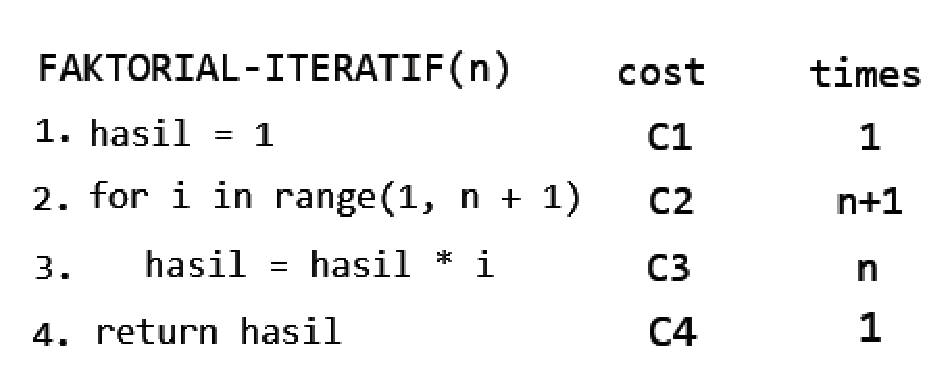
\includegraphics[scale=0.5]{fig/faktorialAnalysis}%
\caption{Analisis Faktorial}%
\label{fig:faktorialAnalysis}%
\end{figure}

\FloatBarrier
Untuk mempermudah perhitungan, biasanya setiap langkah dianggap menghabiskan waktu yang konstan yaitu konstanta $c_i$ dimana $i$ menandakan baris keberapa dari \textit{pseudocode} algoritma tersebut. Nilai dari $c_i$ sendiri tidaklah penting, yang penting adalah berapa kali konstanta $c_i$ itu dieksekusi. Dari Gambar \ref{fig:faktorialAnalysis}, setiap langkah (baris) memiliki biaya (\textit{cost}) eksekusi. 
Biaya eksekusi tersebut dilambangkan dengan besarnya konstanta $c_i$ yang dikalikan banyaknya konstanta tersebut dieksekusi yaitu $n$, dengan kata lain lamanya waktu yang dibutuhkan untuk mengeksekusi setiap langkah adalah $c_{i}\times{}n$ atau disingkat $c_{i}n$

\FloatBarrier
Penjelasan lebih detil dari Gambar \ref{fig:faktorialAnalysis} adalah sebagai berikut.
\begin{enumerate}
	\item Baris 1: Memiliki biaya sebesar $c_1$ dimana biaya tersebut akan diulang sebesar $1$ kali.  
	\item Baris 2: Memiliki biaya sebesar $c_2$ dimana biaya tersebut akan diulang sebesar $n+1$ kali. Pengulangan sebesar $n+1$ kali dikarenakan adanya sebuah looping ``\textbf{for} $i=1$ \textbf{to} $n$''. Looping \textbf{for} akan dieksekusi oleh komputer sebanyak $n+1$ kali. Untuk mempermudah perhitungan maka kita misalkan $n$ bernilai 5, maka baris 2 akan diulang sebanyak 6 kali (1,2,3,4 dan 5 bernilai $True$ dan 1 kali terakhir bernilai $False$) atau $n$+1 kali.
	\item Baris 3: Memiliki biaya $c_{3}$. Ketiga baris tersebut masing-masing diulang sebanyak $n$ kali. Kenapa $n$ kali? Karena semua baris di dalam \textit{looping} \textbf{for} hanya diulang untuk setiap \textbf{for} yang bernilai $True$.
	\item Baris 4: Memiliki biaya 0 karena baris tersebut tidak benar-benar dijalankan oleh program.
\end{enumerate}

Total waktu eksekusi dari Algoritma Faktorial Iteratif dilambangkan dengan $T(n)$ dimana:
\begin{equation}
\label{eq:eksekusiFaktorial1}
T(n) = c_{1} + c_{2}(n+1) + c_3{n} = (c_{2}+c_{3})n + (c_{1}+c_{2}+1)
\end{equation} 

Persamaan \ref{eq:eksekusiFaktorial1} bisa disederhanakan menjadi $T(n)$ = $an$ + $b$. 


Dari persamaan \ref{eq:eksekusiFaktorial1} yaitu $an$ + $b$, terdapat dua konstan ($a$, dan $b$) yang besarnya tergantung pada $c_i$. Untuk membuat lebih sederhana, kita bisa membuat abstraksi yang lebih sederhana yaitu dengan hanya memperhatikan laju pertumbuhan fungsi (\textit{order of growth}). Untuk itu kita cukup hanya perlu memperhatikan order tertinggi dari fungsi yaitu $an$ karena order yang lebih rendah lajut pertumbuhannya tidak begitu signifikan untuk nilai $n$ yang besar. Untuk itu kita tulis bahwa \textit{insertion sort} memiliki waktu eksekusi $\theta(n)$.

\section{Contoh Kasus: Analisis \textit{Bubble Sort}}

Berikut adalah \textit{pseudocode} dari Bubble Sort:

\lstinputlisting[language=Python, caption=Algoritma Bubble Sort]{code/2-bubble-sort.py}

Sebelum menganalisis Algoritma \ref{algo:bubble} ada dua hal penting yang harus dipahami terlebih dahulu: besar masukan (\textit{input size}) dan waktu eksekusi (\textit{running time}). 
\begin{figure}[htbp]%
	\includegraphics[scale=0.6]{fig/BubbleAnalysis}%
	\caption{Analisis \textit{Bubble Sort}}%
	\label{fig:analisisBubbleSort}%
\end{figure}

\FloatBarrier

\lstinputlisting[language=Python, caption=Algoritma Insertion Sort]{code/3-insertion-sort.py}

Penjelasan lebih detil dari Gambar \ref{fig:analisisInsertionSort} adalah sebagai berikut.
\begin{enumerate}
	\item Baris 1: Memiliki biaya sebesar $c_1$ dimana biaya tersebut akan diulang sebesar $n$ kali. Pengulangan sebesar $n$ kali dikarenakan adanya sebuah loop	ing ``\textbf{for} $i=1$ \textbf{to} $A.length-1$''. Looping \textbf{for} akan dieksekusi oleh komputer sebanyak $(A.length-1)+1$ kali.
	\item Baris 2 \& 7: Baris ini diulang sebanyak $\sum\limits_{i=2}^n i$ kali. 
	\item Baris 3 \& 6: Baris ini diulang sebanyak $\sum\limits_{i=1}^{n-1} i$ kali.
	\item Baris 4 - 6: Baris ini diulang sebanyak $\sum\limits_{i=1}^{n-1} t_{i}$ kali.
\end{enumerate} 

Total waktu eksekusi dari Algoritma \ref{algo:insertion} dilambangkan dengan $T(n)$ dimana:
\begin{equation}
\label{eq:eksekusiBubble1}
T(n) = c_{1}n + c_{2}\sum\limits_{i=2}^n i + c_{3}\sum\limits_{i=1}^{n-1} i + (c_{4}+c_{5}+c_{6})\sum\limits_{i=1}^{n-1} t_{i} 
\end{equation} 

Seandainya semua bilangan sudah terurut maka baris ke 4, 5 dan 6 dari Algoritma \ref{algo:insertion} tidak perlu dijalankan lagi karena perintah di baris ke 5 akan selalu menghasilkan $False$. Dengan kata lain nilai dari $t_{i}$ bernilai 0 karena tidak pernah dijalankan. Maka Persamaan \ref{eq:eksekusiBubble1} akan menjadi sebagai berikut.
\begin{eqnarray}
T(n) & = & c_{1}n + c_2((n-1)(n-2))/2+c_3((n-1)n)/2
\label{eq:eksekusiBubble2}
\end{eqnarray}

Persamaan \ref{eq:eksekusiBubble2} merupakan apa yang biasa disebut sebagai \textit{best case} atau kasus terbaik. Jika persamaan tersebut disederhanakan maka bisa ditulis sebagai $an^2+bn+c$. 

Untuk kasus terburuk (\textit{worst case}) akan terjadi jika \textit{array} angka yang akan diurut disusun secara terbalik semua (misalnya mengurut bilangan $\left\{5,4,3,2,1\right\}$ menjadi $\left\{1,2,3,4,5\right\}$). Untuk kasus tersebut, berarti kita harus mencocokkan setiap angka di \textit{inner loop}, atau dengan kata lain nilai dari $t_{i}$ adalah sama dengan nilai dari $i$. 

\begin{eqnarray}
T(n) & = & c_{1}n + c_2((n-1)(n-2))/2+(c_3+c_4+c_5+c_6)(((n-1)n)/2)
\label{eq:eksekusiBubble3}
\end{eqnarray}

Persamaan \ref{eq:eksekusiBubble3} bisa disederhanakan menjadi $an^2+bn+c$ atau yang disebut juga dengan fungsi kuadratic akan $n$. 

Baik \textit{Best Case} dan \textit{Worst Case} sama-sama memiliki nilai $\theta(n^2)$.

\section{Contoh Kasus: Analisis \textit{Insertion Sort}}
Berikut adalah analisis dari Algoritma \ref{algo:insertion}.
\begin{figure}[htbp]%
	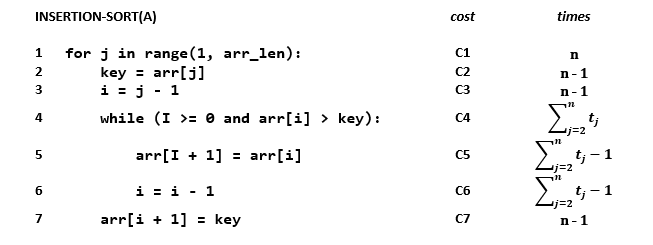
\includegraphics[scale=0.7]{fig/InsertionSortAnalysis}%
	\caption{Analisis \textit{Insertion Sort}}%
	\label{fig:analisisInsertionSort}%
\end{figure}

\FloatBarrier
Penjelasan lebih detil dari Gambar \ref{fig:analisisInsertionSort} adalah sebagai berikut.
\begin{enumerate}
	\item Baris 1: Memiliki biaya sebesar $c_1$ dimana biaya tersebut akan diulang sebesar $n$ kali. Pengulangan sebesar $n$ kali dikarenakan adanya sebuah loop	ing ``\textbf{for} $j=2$ \textbf{to} $A.length$''. Looping \textbf{for} akan dieksekusi oleh komputer sebanyak $A.length+1$ kali. Untuk mempermudah perhitungan maka kita lambangkan $A.length+1$ sebagai $n$. Sebagai contohnya, jika $A.length$ bernilai 5, maka baris 1 akan diulang sebanyak 6 kali (1,2,3,4 dan 5 bernilai $True$ dan 1 kali terakhir bernilai $False$) atau dengan kata lain $n$ bernilai 6.
	\item Baris 2 -- 4: Memiliki biaya masing-masing $c_{2}$, 0, dan $c_{4}$. Baris ke 3 bernilai 0 dikarenakan merupakan komentar yang tidak memakan sumber daya komputer. Ketiga baris tersebut masing-masing diulang sebanyak $n-1$ kali. Kenapa $n-1$ kali? Karena semua baris di dalam \textit{looping} \textbf{for} hanya diulang untuk setiap \textbf{for} yang bernilai $True$.
	\item Baris 5: Baris ini diulang sebanyak $\sum\limits_{j=2}^n t_{j}$ kali. Di baris ini ada dua buah \textit{looping}: \textit{outer loop} -- \textbf{for} dan \textit{inner loop} -- \textbf{while}. Untuk \textit{inner loop} dilambangkan dengan $t_{j}$. $t_{j}$ melambangkan jumlah \textit{looping inner loop}. Ketika \textit{inner loop} dan \textit{outer loop} digabungkan maka menjadi $\sum\limits_{j=2}^n t_{j}$.  
\end{enumerate}                                       
                                     
Total waktu eksekusi dari Algoritma \ref{algo:insertion} dilambangkan dengan $T(n)$ dimana:
\begin{equation}
\label{eq:eksekusiInsertion1}
T(n) = c_{1}n + c_{2}(n-1) + c_{4}(n-1) + c_{5}\sum\limits_{j=2}^n t_{j} + c_{6}\sum\limits_{j=2}^n (t_{j}-1) + c_{7}\sum\limits_{j=2}^n (t_{j}-1) + c_{8}(n-1) 
\end{equation} 

Dari Persamaan \ref{eq:eksekusiInsertion1}, kita bisa menghitung total waktu eksekusi ($T(n)$) yang bergantung kepada variabel $n$ atau banyaknya bilangan masukan. Semakin banyak bilangan masukan maka $T(n)$ akan semakin tinggi dan sebaliknya. Akan tetapi, $T(n)$ tidak hanya bergantung pada banyaknya bilangan masukan, tetapi bergantung juga kepada susunan bilangan tersebut. Bagaimana jika \textit{array} bilangan tersebut sudah terurut? Bukankah waktu yang dibutuhkan akan lebih sedikit dibandingkan jika semua bilangan tersebut terbalik urutannya?

Seandainya semua bilangan sudah terurut maka baris ke 6 dan baris ke 7 dari Algoritma \ref{algo:insertion} tidak perlu dijalankan lagi karena perintah di baris ke 5 akan selalu menghasilkan $False$. Dengan kata lain nilai dari $t_{j}$ akan selalu konstan yaitu 1. Maka Persamaan \ref{eq:eksekusiInsertion1} akan menjadi sebagai berikut.
\begin{eqnarray}
T(n) & = & c_{1}n + c_2(n-1)+c_4(n-1)+c_5(n-1)+c_8(n-1)
\nonumber \\
 & = & (c_1+c_2+c_4+c_5+c_8)n-(c_2+c_4+c_5+c_8)
\label{eq:totalEksekusi3}
\end{eqnarray}

Persamaan \ref{eq:eksekusiInsertion1} merupakan apa yang biasa disebut sebagai \textit{best case} atau kasus terbaik. Jika persamaan tersebut disederhanakan maka bisa ditulis sebagai $an+b$ atau yang biasa disebut sebagai fungsi linear akan $n$. 

Untuk kasus terburuk (\textit{worst case}) akan terjadi jika \textit{array} angka yang akan diurut disusun secara terbalik semua (misalnya mengurut bilangan $\left\{5,4,3,2,1\right\}$ menjadi $\left\{1,2,3,4,5\right\}$). Untuk kasus tersebut, berarti kita harus mencocokkan setiap angka di \textit{inner loop}, atau dengan kata lain nilai dari $t_{j}$ adalah sama dengan nilai dari $j$ yang berasal dari \textit{outer loop}. 

\begin{eqnarray}
T(n) & = & c_1n + c_2(n-1) + c_4(n-1) + c_5(\frac{n(n+1)}{2}-1) + c_6(\frac{n(n-1)}{2})   \nonumber \\ 
& & + c_7(\frac{n(n-1)}{2})+c_8(n-1) 
\nonumber \\ 
 & = & (\frac{c_5}{2}+\frac{c_6}{2}+\frac{c_7}{2})n^2+(c_1+c_2+c_4+\frac{c_5}{2}-\frac{c_6}{2}-\frac{c_7}{2}+c_8)n \nonumber\\
& & -(c_2+c_4+c_5+c8)
\label{eq:eksekusiInsertion2}
\end{eqnarray}

Persamaan \ref{eq:eksekusiInsertion2} bisa disederhanakan menjadi $an^2+bn+c$ atau yang disebut juga dengan fungsi kuadratic akan $n$. 

Dari persamaan \ref{eq:eksekusiInsertion2} yaitu $an^2+bn+c$, terdapat tiga konstan ($a$, $b$, dan $c$) yang besarnya tergantung pada $c_i$. Untuk membuat lebih sederhana, kita bisa membuat abstraksi yang lebih sederhana yaitu dengan hanya memperhatikan laju pertumbuhan fungsi (\textit{order of growth}). Untuk itu kita cukup hanya perlu memperhatikan order tertinggi dari fungsi yaitu $an^2$ karena order yang lebih rendah lajut pertumbuhannya tidak begitu signifikan untuk nilai $n$ yang besar. Untuk itu kita tulis bahwa \textit{insertion sort} memiliki \textit{worst case} $\theta(n^2)$.
